%------------------------------------------------------------
\documentclass[conference,letterpaper]{IEEEtran}
\usepackage[spanish]{babel}
\usepackage[utf8]{inputenc}
\usepackage{amsmath}
\usepackage{amssymb}
\usepackage[usenames]{color}
\usepackage[pdftex]{graphicx}
\usepackage{tcolorbox}
\usepackage[colorlinks, linkcolor=black]{hyperref}
\tcbuselibrary{listingsutf8}
%------------------------------------------------------------
\graphicspath{{../pdf/}{../jpeg/}}
\DeclareGraphicsExtensions{.pdf,.jpeg,.png}
%------------------------------------------------------------
\hyphenation{op-tical net-works semi-conduc-tor}
%------------------------------------------------------------
\definecolor{Fucsia}{RGB}{193,124,250}
\definecolor{Azul}{RGB}{20,80,200}
%------------------------------------------------------------
\DeclareRobustCommand*{\IEEEauthorrefmark}[1]{\raisebox{0pt}[0pt][0pt]{\textsuperscript{\footnotesize #1}}}
%------------------------------------------------------------
% Definir cuadro de ancho del texto
\newtcolorbox{mybox}[1]{colback=red!5!white,colframe=red!75!black,fonttitle=\bfseries,title=#1}
%------------------------------------------------------------
% Cuadro estrecho
\newtcbox{cuadro}[1]{colback=blue!5!white,colframe=blue!75!black,fonttitle=\bfseries,title=#1}
%------------------------------------------------------------
% Cuadro numerado para ejemplos
\newtcolorbox[auto counter,number within=section]{example}[2][]
{colback=green!5!white,colframe=green!75!black,fonttitle=\bfseries, title=Ejemplo~\thetcbcounter: #2,#1}
%------------------------------------------------------------
\begin{document}

\title
{
An\'alisis de Round Robin para sistemas de multiprocesadores
}

\author
{
\IEEEauthorblockN
{
C\'ondor Torres Jes\'us \'Angel.\IEEEauthorrefmark{1},
Lazon Vera, Erick.\IEEEauthorrefmark{2} 
}                                     
\IEEEauthorblockA
{
jcondort@uni.pe \IEEEauthorrefmark{1},
elazon@uni.pe \IEEEauthorrefmark{2}
}
\IEEEauthorblockA
{
Universidad Nacional de Ingeniería, Rimac, Lima, Perú}
}

\maketitle

\begin{abstract}
Si bien en sus inicios los computadores contaban con una arquitectura de solo con un procesador, en la actualidad es muy común ver sistemas de multiprocesadores y su tendencia a este tipo de sistema es a extenderse y evolucionar, por ejemplo, ya podemos observarlas en nuestras máquinas de escritorio, laptops e incluso en nuestros smartphones (que incluso cuentan con unidades multinúcleo dedicadas a la inteligencia artificial). El rendimiento comparado a los procesadores monon\'ucleo ha hecho que proliferen en distintos sistemas, sin embargo junto con los beneficios han aparecido dificultades entre algunas de ellas complejas, la primera es adaptar software que ya funcionaba en un solo núcleo para aprovechar todos los núcleos del sistema empleando hilos (programación paralela). Por otro lado surge la necesidad que dichos sistemas multiprocesadores gestionen de manera adecuada los recursos y los tiempos de cada procesador. En esta ocasión estudiaremos el comportamiento de un planificador Round Robin para un sistema multiprocesador.
\end{abstract}

%{\smallskip \keywords controlador PID, estándar OPC, función de transferencia.}

\IEEEpeerreviewmaketitle

\vspace{7pt}
\section{Introducción}
En un sistema inform\'atico tipico existen muchos procesos concurrentes que compiten por recursos, para esto el sistema operativo debe manejar la asignación de recursos de forma eficiente y con respectivo cuidado. El mayor desafío de estos sistemas es establecer planificadores adecuados, un planificador impacta directamente en el rendimiento de un sistema pues es quien se encarga de asignar tiempos de uso del procesador y recursos para la ejecución. Primero debemos familiarizarnos con algunos términos:

\subsection{Multiprogramaci\'on}
Planteamos la siguiente situación, en una oficina de correos un usuario X se une a una cola de atención para recibir su pedido, luego de un tiempo transcurrido finalmente llega su turno, pero su envío aún no está preparado para su despacho entonces lo pasan a un lado a la espera que su envío sea empacado mientras tanto otro cliente es atendido, esta idea aunque simple nos permite mostrar  la idea básica de la multiprogración que se busca que la atención no se detenga sino que se fluya a pesar de estos tipos de incovenientes.\\

An\'{a}logamente al ejemplo anterior, algo muy similar ocurre con  el  concepto  de  multiprogramaci\'{o}n,  por  ejemplo,  en  un sistema  operativo  cuando  hay  uno  o  m\'{a}s  programas  listos para  ejecutarse  en  la  memoria  principal,  como  la  CPU  s\'{o}lo puede  hacer  la  ejecuci\'{o}n  de  un  programa,  la  idea  es  tener un  sistema  multiprogramado  para  que  se  pueda  optimizar  el tiempo del CPU. El sistema operativo puede tener varios tipos de  interrupciones  como  la  espera  de  IO,  el  transferimiento de  control  a  otro  cliente  entre  otros,  por  eso  uno  de  los objetivos   de   la   multiprogramaci\'{o}n   es   que   los   procesos que  esperan  IO  no  deban  bloquear  otros  procesos  que  a  su vez generan m\'{a}s desperdicio de tiempo haci\'{e}ndolo ineficiente.\\

Hay que tener en cuenta tambi\'{e}n los problemas que puede abordar  el  cargar  varios programas  en  la  memoria  principal como  lo  es  fragmentaci\'{o}n  o  tambi\'{e}n  cuando  un  programa sea m\'{a}s grande que la memoria( lo cual se puede solucionar a  trav\'{e}s  del  uso  de  la  memoria  virtual).  En  resumen  la multiprogramaci\'{o}n  permite  que  m\'{u}ltiples  procesos  residan en  la  memoria  principal  y  tiene  como  objetivo  principal optimizar  la  utilizaci\'{o}n  de  la  CPU  reduciendo  el  tiempo  de inactividad de esta.\\

\subsection{Multiprocesamiento}
Se  refiere a  las  unidades de  CPU  que  el  sistema  puede contar,  si  el  hardware  proporciona  m\'{a}s  de  un  procesador,entonces  usamos  el  t\'{e}rmino \textbf{Multiprocesamiento},  puede  haber  variaciones  en  el  esquema  b\'{a}sico  como  tener  m\'{u}ltiples n\'{u}cleos, dados o paquetes en el sistema.



\subsection{Multitarea}
Este termino es usado en los sistemas operativos modernos en el cual se refiere cuando varias tareas comparten un recurso de procesamiento comun, tambien se refiere a la ilusion de paralelismo cuando la CPU reasigna a otra tarea (cambio de contexto), hay que tener en cuenta que una tarea en un sistema multitarea no es un programa de aplicacion completo ya que los sistemas operativos modernos cuentan con su division en paginas logicas. Se puede decir que la multitarea y la multiprogramacion tienen un concepto similar la cual es el compartimiento del tiempo del CPU.

\subsection{Multi Threading}
Para este termino primero veamos el concepto de subprocesamiento la cual es un modelo de ejecucion que permite que un solo proceso tenga multiples subprocesos. El subprocesamiento multiple es una forma de escribir software concurrente aunque tambien hay que tener en cuenta la sincronizacion de subprocesos.

\subsection{Tiempo compartido}
Los sistemas operativos de programación múltiple y multitarea son estructuras de sistemas de tiempo compartido. En la programación múltiple, aunque la CPU se comparte entre los programas, no es una estructura eficiente para compartir el tiempo de la CPU debido a que el programa sigue ejecutándose hasta que se bloquea, por otro lado, en una estructura de multitarea, el tiempo compartido tiene una mejor eficiencia porque cada proceso de ejecución solo toma un tiempo justo cantidad del tiempo de CPU llamado tiempo cuántico. Incluso en un sistema de multiprocesamiento cuando tenemos más de un procesador, cada tiempo de procesador se comparte entre los procesos en ejecución. Por eso podemos ver que todos los términos están relacionados de alguna manera u otra, sin embargo, no usar el término correcto en el contexto correcto es lo que hace que genere la confusion de terminos. 

\subsection{Sistema de tiempo real}
 En un sistema de tiempo compartido, los procesos del sistema operativo se programan para que el tiempo de CPU se comparta entre todo el grupo. Dependiendo del algoritmo de programación, cada proceso obtiene su parte del tiempo de CPU, pero no hay garantía de que un proceso obtenga la CPU cuando lo desee. Tambien hay que tener en cuenta que en un sistema en tiempo real, un proceso garantiza la atención de la CPU cuando ocurre un evento específico, por lo tanto debe haber un tiempo límite operativo desde el momento en que se activa el evento hasta el momento en que el sistema responde, es por eso que se dice que los procesos de un sistema en tiempo real son de misión crítica. Un ejemplo practico es el caso de los robots industriales en una línea de ensamblaje, donde se espera que en cada etapa tenga lugar una determinada operación.\\
 
\section{Organizaci\'on del informe (Secciones)}
Para esta seccion presentaremos los algoritmos o soluciones (secciones) que tendra nuestro informe final, por ahora solo mencionaremos los metodos que podemos proponer. Primeramente nuestro proyecto consistira de un distribuidor de cargas aciclica, osea un servidor llamado "Maestro" que distribuira entre los otros procesadores (esclavos). Las formas de distribuir pueden ser de distintas formas, algunas de ellas puden ser:

\subsection{Metodo Round Robin}
Es un metodo que selecciona un grupo de manera equitativa y en orden racional, que recorre desde el primero hasta el ultimo y si no se finalizaron los trabajos, se vuelve a repetir el ciclo hasta que terminen todos los trabajos, una caracteristica principal de este m\'etodo es el uso del \textbf{quantum}, el cual es un numero fijo de pulsos o ciclos de reloj, debido a esto el quantum debe fijarse en un cierto tamaño de modo que la mayoria de peticiones o trabajos requieran menos tiempo que la duracion del cuanto. Otras caracteristicas que puede presentar son:

\begin{itemize}
    \item Cuando se genera una interrupcion, el proceso que esta en ejecucion se traslada a una cola de lista y se selecciona el siguiente trabajo.
    \item Esta diseñado especialmente para sistemas de tiempo compartido.
    \item Para un parametro critico, su efectividad dependera del tamaño del cuanto pero hay que tener en cuenta el tiempo que se dedica al cambio de contexto
\end{itemize}

\begin{figure}[thpb]
      \centering
      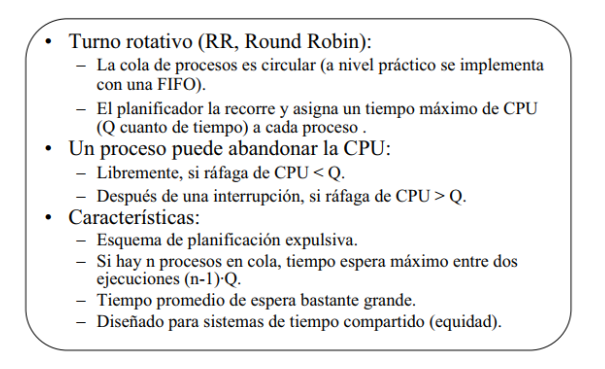
\includegraphics[width=0.6\linewidth]{rr.png}
      \caption{Funcionamiento de Round Robin.}
      \label{fig:RR}
\end{figure}

Los conceptos a tener en cuenta en el algoritmo de este metodo son:
\begin{enumerate}
    \item \textbf{Quantum}: Numero maximo de intervalos de tiempo que un proceso puede usar la CPU.
    \item \textbf{Tiempo de llegada}: Intervalo de tiempo en que comienza el proceso.
    \item \textbf{Tiempo de ejecucion o Rafaga}: Intervalo de tiempo que demora un proceso en ejecutarse.
    \item \textbf{Tiempo de finalizacion}: Intervalo de tiempo en que termina el proceso.
    \item \textbf{Tiempo de retorno}: Suma de intervalos que mide desde que comienza el proceso hasta que finaliza su ejecucion.
\end{enumerate}

\subsection{Tablas Hash}
Otro proposicion que podriamos hacer, pero no asegurar es la utilizacion de tablas hash, la cual es un contenedor asociativo que permite el almacenamiento de entradas con una clave unica para luego ser recuperadas posteriormente de manera eficiente, debido a que la clave es unica para cada entrada entonces se puede usar a esta clave como un identificador.

Su estructura hace que la recuperacion de informacion sea eficiente con un tiempo constante, sin embargo, esta tabla hash frecuentemente se producen colisiones, esto se pasa generalmente cuando una clave se genera para dos entradas, sin embargo esto tiene solucion gracias a que ya cuenta con una funcion de resoluciones de colisiones, por eso existen dos tipos de tablas hash en funcion a como se resulven sus colisiones:

\begin{itemize}
    \item Encadenamiento separado: Las colisiones se resuelven insertandolas en una lista.
    \item Direccionamiento abierto: Se usa un vector como representacion y cuando ocurre la colision, le volvemos a reasignar otra clave no repetida.
\end{itemize}

\begin{figure}[thpb]
    \centering
    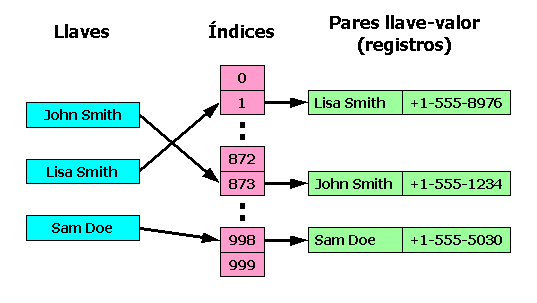
\includegraphics[width=0.55\linewidth]{Tabla_hash1.png}
    \caption{Caption}
    \label{fig:hash}
\end{figure}

Las operaciones que se pueden utilizar en una tabla hash son:
\begin{itemize}
    \item Insertar: Puede ser un valor entero o una cadena de caracteres.
    \item Borrar: Si uno quiere borrar un nodo debe seleccionar dicho nodo.
    \item Vaciado de lista: Elimina todos los elementos de la tabla
\end{itemize}

\subsection{Teor\'ia de Colas}
Una de las herramientas que se utilizan en los sistemas multiprocesadores es el uso de colas, la cual se define como un fen\'omeno matem\'atico y tiene una gran cantidad de aplicaciones en diferentes ramas como Ciencias M\'edicas, Ciencias de la Gesti\'on, Sistemas inform\'aticos y econometria. Segun el modelo de teor\'ia de colas, esta surge con el prop\'osito de predecir algunas medidas de rendimiento en la computadoras, ya que esta se enmarca en estimar los tiempos de espera y la longitud de la cola. Segun la teor\'ia de colas que pertenece a la rama de Investigaci\'on de operaciones, estas utilizan los recursos para ofrecer el servicio dependiendo de la decision comercial que pueda tener el modelo. Para estos modelos existen \textbf{Sistemas Multiservidor de cola m\'ultiple} y el \textbf{Sistema de cola de Servidor \'unico de cola m\'ultiple}, ambas cuentan con las siguientes caracter\'isticas:

\begin{itemize}
    \item Promedio de la tasa de llegada.
    \item Promedio de la tarifa de servicio.
    \item Eficiencia del sistema.
    \item N\'umero de clientes existentes en la cola.
    \item N\'umero de clientes en el sistema.
    \item Tiempo de espera del cliente en la cola.
    \item Tiempo de espera del cliente en el sistema.
\end{itemize}

\section{Estado del Arte}
En el planteamiento de este proyecto, ademas de las herramientas que tenemos a nuestra disposicion, debemos usar metodos que nos ayuden incrementar la eficiencia del sistema, entre estos tenemos los algoritmos de planificacion los cuales sobresalen los siguientes:

\begin{enumerate}
    \item \textbf{Algoritmo de planificacion basado en timestamp}.
    \item \textbf{Algoritmo de planificacion basado en Round Robin}.
    \item \textbf{Algoritmos hibridos}
\end{enumerate}

Debido a que nos enfocamos en el segundo tipo de algoritmo de planificacion veamos como funciona, para empezar este algoritmo asigna una ranura de tiempo a cada flujo y hace que los envios de paquetes sea de forma alternada, Por ejemplo, si se tuvieran 3 colas (Q1, Q2 y
Q3) a cada una de estas colas se le asigna una ranura de tiempo de duración tiempo t1, entonces el algoritmo comenzaria a enviar los paquetes de Q1 durante el tiempo t1, luego de eso comienza a enviar paquetes de la cola Q2 durante el mismo tiempo y finamente envia paquetes de la cola Q3 durante un mismo tiempo y si aun no termina los paquetes vuelve de nuevo a la cola Q1 y asi hasta que se acabe los paquetes de las tres colas. A pesar que Round Robin tiene una mejor distribucion de los labores, tiene una respuesta muy pobre con respecto al retraso de cada paquete obtenido.

\subsection{Weight Round Robin (WRR)}
Este algoritmo es una modificacion del Round Robin en el cual solo se envia un paquete por cola en cada turno, este funcionamiento se da por cada flujo en el cual se le da un peso en parte de ancho de banda, entonces, el número de paquetes a enviar en cada turno se calcula con base en el peso del flujo y en la capacidad del enlace.

WRR funciona bien en el envío de paquetes de tamaño fijo, sin embargo,
presenta problemas de desempeño en los paquetes que son de longitud variable, por ejemplo, en el caso de paquetes de tamaño mayor, este utiliza más ancho de banda de lo que deberia asignarse, lo cual hace que el desempeño en el envío de paquetes de las otras colas disminuya, un ejemplo claro de este tipo de algoritmo encontramos en los dispositivos de interconectividad Huawei en los cuales se manejan ocho colas en el que se les asigna un determinado porcentaje de ancho de banda.

\subsection{Deficit Round Robin}
Este algoritmo mejora las dificultades de WRR y ahora permite enviar paquetes de diferentes longitudes, tiene dos variables, una es el \textbf{quantum} que indica la cantidad de bits a enviar en cada turno y la otra variable es el \textbf{contador de deficit} que se encarga de almacenar el valor del quantum obtenido.

El funcionamiento de este algoritmo comienza enviando paquetes de colas que tengan por mandar, si el tamaño de este paquete es menor o igual al valor del quantum, el paquete es enviado sino el paquete debe esperar a ser transmitido a otro turno, es ahi donde entra el deficit counter, lo que hace iniciar su cola e incrementa su valor por cada paquete que no es enviado debido a la condicional del quantum, cuando el deficit counter llega a su tope o limite de paquetes estas son enviadas a procesarse y el deficit counter vuelve a cero


De acuerdo con algunos articulos cientificos el metodo Round Robin es utilizado en modelos de metodologia empirica, la cual propone un modelo matematico en una comparacion de un evento con su numero de participantes (ejemplo de una liga de futbol con su numero de participantes).

\begin{figure}[thpb]
    \centering
    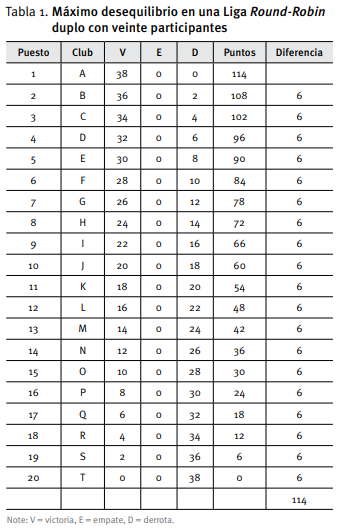
\includegraphics[width=0.55\linewidth]{tabla.png}
    \caption{Resultados de un metodo doble Round Robin}
    \label{fig:tabla}
\end{figure}

Considerando el ejemplo anterior donde se utiliza el metodo doble Round Robin, el analisis de este ejemplo considera que en todo torneo o liga hay un porcentaje de desequilibrio en el balance competitivo. Algunos investigadores destacan la posibilidad de utilizar metodos estadisticas para buscar diferencias significativas entre las medias de los distintos torneos.

\section{Metodolog\'ia o diseño del proyecto}
El proyecto consiste en la distribucion de cargas a traves de un proceso Servidor (maestro) y los otros procesos seran aquellos que  trabajen las cargas (esclavos), para plasmar esta idea en codigo se propone hacerlo en lenguaje java donde se compondra de dos partes:

\begin{itemize}
    \item \textbf{Servidor}: Se encargara de la distribucion de tareas o cargas, ademas vera que los todos los procesos esten ejecutando correctamente.
    \item \textbf{Cliente}: Se encargara de la ejecucion de las tareas que se den y una vez resuelta esta devolvera al servidor.
\end{itemize}

El programa Servidor - cliente estara codificado en lenguaje java utilizando la herramienta de los sockets para la comunicacion, ya que esto nos permite mandar mensajes a otras maquinas a traves de la conexion TCP, eso quiere decir que el servidor esperara que los "esclavos" respondan para que puedan procesar sus tareas, dependiendo de lo que el Servidor les mande hacer.
\section{Conclusiones}
Se propuso la estructura y forma del proyecto, los cuales estaran en constantes pruebas para obtener una buena distribucion de cargas.\\

Se propuso los metodos de Round Robin y Tabla Hash para que los procesos puedan tener una mejor eficiencia en la distribucion y ejecucion de tareas.\\

Se mostro un modelo ejemplo de como se puede utilizar el metodo Round Robin para un caso real con probabilidades.

\begin{thebibliography}{1}
\normalsize
\bibitem{}
Franck, E. (2014), \emph{Financial fair play in European football clubs: What is it all about? International Journal of Sports Finance, 9(3), 193-217.}
\\
\bibitem{}
Haan, M., Koning, R. H., & Witteloostuijn, A. (2007), \emph{Competitive balance in national European soccer competitions. In J. Albert, R. H. Koning (Eds.). Statistical thinking in sports (Chap. 4, pp. 63-76). London: Taylor and Francis.}
\\
\bibitem{}
Levin, R., Mitchell, G., Volcker, P. Will, G. (2000), \emph{The report of the independent members of the Comissioners Blue Ribbon Panel on baseball economics},\\ Recuperado en: 
\url{http://www.mlb.com/mlb/downloads/blue\_ribbon.pdf}
\\
\bibitem{}
Zhiwen Chen, \emph{ student at the College of Computer Science and Electronic Engineering, Hunan University, China. His research interests are in parallel computing and multi-core systems.} 
\\
\bibitem{}
Jianhua Sun, \emph{Associate Professor at the College of Computer Science and Electronic Engineering, Hunan University, China. She received the Ph.D. degree in Computer Science from Huazhong University of Science and Technology, China in 2005. Her research interests are in security and operating systems. She has published more than 70 papers in journals and conferences, such as IEEE Transactions on Parallel and Distributed Systems}, IEEE Transactions on Computers.
\\
\bibitem{}
Víctor M. Alfaro Ruíz, \emph{Métodos de sintonización de controladores PID que operan como reguladores}, San José, Costa Rica, 2002.\\ Disponible en: 
\url{http://eie.ucr.ac.cr/uploads/file/documentos/pub_inv/articulos/valfaro02B.pdf}

\bibitem{}
Knightson, K. Morita, N., Towle T. NGN Architecture: Generic \emph{Principles, Funcional Architecture, and Implementation. IEEE Communications Magazine}. Octubre 2005.
\end{thebibliography}
\end{document}